
\mysection{Дискретные вероятностные пространства}

В дискретном случае множество элементарных исходов $\Omega$ -- счетно или конечно.

Сигма-алгебру $\setF$ на $\Omega$ выбирают дискретной, $\setF = \setF^* = 2^\Omega$

Тогда вероятность $P$ можно задать как функцию на $\Omega$:
\begin{multline*}
	\shoveright{P\colon \Omega \to [0, 1],\; \text{т.ч. } \sum_{\omega \in \Omega} P(\omega) = 1}
\end{multline*}

В этом случае $\forall A \subset \Omega$ : $P(A) = \sum\limits_{\omega \in A} P(\omega)$

\begin{enumerate}[label=\protect\circled{\Roman*},series=models]
	\item \bigtitle{Классическая модель}
\end{enumerate}

В классической модели $\Omega$ -- конечно, все элементарные события равновероятны:
\begin{multline*}
	\shoveright{\forall \omega \in \Omega : P(\omega) = \frac{1}{|\Omega|}}
\end{multline*}

Тогда $\forall A \subset \Omega$ : $P(A) = \dfrac{|A|}{|\lefteqn{\Omega}\phantom{A}|}$\\

\begin{example}~

	\begin{enumerate}
		\item 
			Бросок монеты.\quad $\Omega$ = \{Орел, Решка\}.\\
			$P$(Орел) = $P$(Решка) = $1/2$
	
		\item 
			Бросок кости.\quad $\Omega = \braces{1, \ldots, 6}$\\
			$P(i) = 1/6\quad \forall i = 1 \ldots 6$
		
		\item 
			Бросок двух монет. "Заблуждение Даламбера". \quad $\Omega = \braces{OO, OP, PP}$\\
			Кажется, что все исходы имеют верятность $1/3$
		
			Проблема в различимости монет.\\
			Если они различимы, то 
			$\Omega = \braces{OO, OP, PO, PP}$,\; и вероятности событий равны $1/4$\\
			$P$(выпал 1 орел и 1 решка) = $1/2$
		
		\item 
			Схема испытаний Бернулли. \quad
			$\Omega = \condset{\vec{\omega} = (w_1, \ldots, w_n)}{w_i \in \braces{0, 1} } $.
			$|\Omega| = 2^{n}$
		
		Эта модель отвечает броскам $n$ различимых монет.
		
	\end{enumerate}

\end{example}

\begin{enumerate}[resume*=models]
	\item \bigtitle{Геометрические вероятности}
\end{enumerate}

Здесь $\Omega \subseteq \setR^n$, $n \geq 1$ и для $\Omega$ определен, конечен и положителен его объем $\mu(\Omega) > 0.$

Сигма-алгебра $\setF$ состоит из тех $A \subset \Omega$ для которых тоже определен объем $\mu(A)$

Тогда вероятность $P$ задается так:
\begin{equation*}
	P(A) = \frac{\mu(A)}{\mu(\Omega)}
\end{equation*} 

Подобная модель -- ествественное продолжение классической модели на случай непрерывных пространств.

\begin{example}
	Задача о встрече:
	
	Два товарища договорились встретиться утром на остановке. Каждый приходит в случайное время между 9 и 10, ждет 15 минут, потом уезжает.

	Какова вероятность встречи?\\

	\begin{solution}
		Пространство элементарных событий -- это квадрат $[9, 10] \times [9, 10]$.

		Время прихода вервого и время прихода второго --- случайная точка $(u, v) \in [9, 10] \times [9, 	10]$.

		Изобразим пространство событий геометрически:

		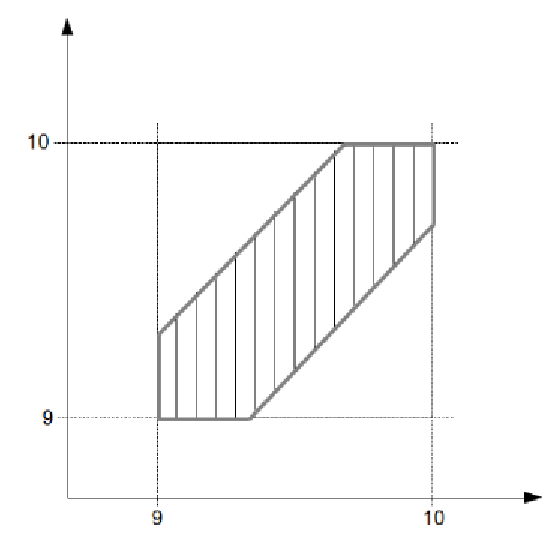
\includegraphics{pictures/13_09_graph.eps}

		Заштрихованная область $A = \condset{(u, v)}{u, v \in [9; 10],\; |u - v| < 1/4 }$.

		Нужно найти меру этой области:

		\begin{align*}
			&\mu(A) = 1 - (3/4)^2 = 7/16\\
			&\mu(\Omega) = 1\\
			&\Rightarrow P(\text{они встретятся}) = \mu(A) / \mu(\Omega) = 7/16\\
		\end{align*}

	\end{solution}
\end{example}

\mysection{Условные вероятности}

Пусть $(\Omega, \setF, P)$ -- вероятностное пространство.

\begin{definition}
	Для $\forall A \in \setF$, т.ч. $P(A) > 0$
	\emph{условной вероятностью} события $B \in \setF$ при условии $A$ называют
	\begin{equation*}
		P(B \mid A) = \frac{P(A \cap B)}{P(A)}
	\end{equation*}
	если же $P(A) = 0,$ то $P(B \mid A) = 0,\; \forall B \in \setF$
\end{definition}

\begin{exercise}
	Если $P(A) > 0$, то функция
	$\comp{P}(B) = P(B \mid A)$
	
	тоже является вероятностной мерой на $(\Omega, \setF)$.
\end{exercise}

\begin{definition}
	Систему событий $\braces{B_n}_{n = 1}^{\infty}$ называют разбиением множества $\Omega$, если:
	\begin{enumerate}
		\item $\forall i \neq j : B_i \cap B_j = \emptyset$
		\item $\bigsqcup\limits_{n = 1}^{\infty} B_n = \Omega$ 
	\end{enumerate}
	
	В этом случае также говорят, что $\braces{B_n}_{n = 1}^{\infty}$ обрезует полную группу несовместных событий.
\end{definition}

\begin{lemma}[формула полной вероятности]~

	Пусть $\braces{B_n}_{n = 1}^{\infty}$ - разбиение $\Omega$. Тогда для $\forall A \in \setF$:
	\begin{equation*}
		P(A) = \sum_{n = 1}^{\infty} P(A \mid B_n) P(B_n)
	\end{equation*}

	\begin{proof}
		Рассмотрим событие $A$
		\begin{align*}
			&P(A) = P(A \cap \Omega) = P\pars{A \cap \bigsqcup_{n = 1}^{\infty} B_n} =
			P\pars{\bigsqcup_{n = 1}^{\infty} A \cap B_n} = \\
			&= \expl{счетная аддитивность} = \sum_{n = 1}^{\infty} P(A \cap B_n) = 
			\sum_{n = 1}^{\infty} P(A \mid B_n) P(B_n)
		\end{align*}
	\end{proof}
\end{lemma}

\begin{example}
	В ящике всего $n$ шаров, из них $k$ - белых. Последовательно, без возвращения, вынимаем по одному шару. 
	Обозначим $A_j$ = \{на $j$-том шаге вынули белый шар\}.

	Доказать:
	\begin{equation*}
		P(A_j) = \frac{k}{n}\\
	\end{equation*}
	
	Первое решение: воспользоваться симметрией.
	
	Второе решение: в лоб

	Введем события $B_j(i)$ = \{среди первых $j - 1$ шара вынули ровно $i$  белых\}\\
	Тогда $B_j(i)$ образуют разбиение, $i = 0 \ldots k$
	
	Легко видеть, что
	\begin{align*}
		&P(A_j \mid B_j(i)) = \frac{k - i}{n - j + 1}\\\\
		&P(B_j(i)) = \comb{j - 1}{i} \frac{ k  (k - 1)  \ldots  (k - i + 1)(n - k) \ldots (n - k - j + 1 + i)}{n(n-1)\ldots (n - j + 1)} = \\
		&= \frac{\comb{j - 1}{i} \comb{k}{i}\, i!\, \comb{n-k}{j-1-i} (j - i - 1)!}{\comb{n}{j - 1} (j-1)!} = \frac{\comb{k}{i} \comb{n - k}{j - 1- i}}{\comb{n}{j - 1}}
	\end{align*}
	
	Отсюда:
	
	\begin{equation*}
		P(A_j) = \sum_{i = 0}^{k} \frac{k - i}{n - j + 1} \frac{\comb{k}{i} \comb{n - k}{j - 1- i}}{\comb{n}{j - 1}} \\
		= \frac{k}{n} \sum_{i = 0}^{k} \frac{\comb{k - 1}{i} \comb{n - k}{j - 1- i}}{\comb{n - 1}{j - 1}} = \frac{k}{n}\\\\
	\end{equation*}

\end{example}

\begin{lemma}[формула Байеса]~

	Пусть $\braces{B_n}_{n = 1}^{\infty}$ -- разбиение $\Omega$, а $A \in \setF : P(A) > 0.$ Тогда $\forall n$
	\begin{equation*}
		P(B_n \mid A) = \frac{P(A \mid B_n) P(B_n)}{\sum_{k = 1}^{\infty} P(A \mid B_k) P(B_k)}
	\end{equation*}
\end{lemma}

\begin{definition}
	$P(B_n)$ называется \emph{априорной вероятностью}.\\
	$P(B_n \mid A)$ называется \emph{апостериорной вероятностью} (относительная вероятность при условии известного результата эксперимента)
\end{definition}

\mysection{Системы множеств}

Пусть $\Omega$ - некоторое множество

\begin{definition}
	Система подмножеств $\setM$ множества $\Omega$ называется \emph{$\pi$ - системой}, \\
	если $\forall A, B \in \setM$ выполнено $A \cap B \in \setM$
\end{definition}

\begin{definition}
	Система подмножеств $\setL$ множества $\Omega$ называется \emph{$\lambda$ - системой}, если
	\begin{enumerate}
		\item 
			$\Omega \in \setL$

		\item 
			Если $A, B \in \setL$ и $A \subset B$, то $B \setminus A \in \setL$

		\item 
			Если последовательность $\braces{A_n}_{n=1}^{\infty}, A_n \in \setL \quad \forall n,$ \\
			удовлетворяет $A_n \uparrow A$ (т.е $A_n \subset A_{n + 1} \subset \ldots$  
			и $A = \bigcup\limits_n A_n$), то $A \in \setL$
	\end{enumerate}
\end{definition}

